\documentclass{article}%
\usepackage[T1]{fontenc}%
\usepackage[utf8]{inputenc}%
\usepackage{lmodern}%
\usepackage{textcomp}%
\usepackage{lastpage}%
\usepackage{graphicx}%
%
\usepackage[sorting=none]{biblatex}%
\addbibresource{../austcovid.bib}%
\title{Supplemental Appendix}%
%
\begin{document}%
\normalsize%
\maketitle%
\section{General model construction}%
\label{sec:Generalmodelconstruction}%
The base model consists of three states, representing fully susceptible, infected (and infectious) and recovered persons. The model is run from 2021{-}08{-}22 to 2022{-}06{-}10. %
The simulation starts with 26.0 million susceptible persons only, with infectious persons only introduced through strain seeding as described below. %
The infection moves people from the susceptible compartment to the infectious compartment, under the frequency{-}dependent transmission assumption. %
The recovery process moves people directly from the infectious state to the recovered compartment, with the rate of transition calculated as the reciprocal of the infectious period.%
Modelled notifications are calculated as the absolute rate of infection in the community multiplied by the case detection rate. %
We took unadjusted estimates for interpersonal rates of contact by age from the United Kingdom data provided by Mossong et al.'s POLYMOD study \cite{mossong2008}. The data were obtained from https://doi.org/10.1371/journal.pmed.0050074.st005 on 12th February 2023 (downloaded in their native docx format). The matrix is transposed because summer assumes that rows represent infectees and columns represent infectors, whereas the POLYMOD data are labelled `age of contact' for the rows and `age group of participant' for the columns.

%
\section{Age stratification}%
\label{sec:Agestratification}%


\begin{figure}%
\centering%
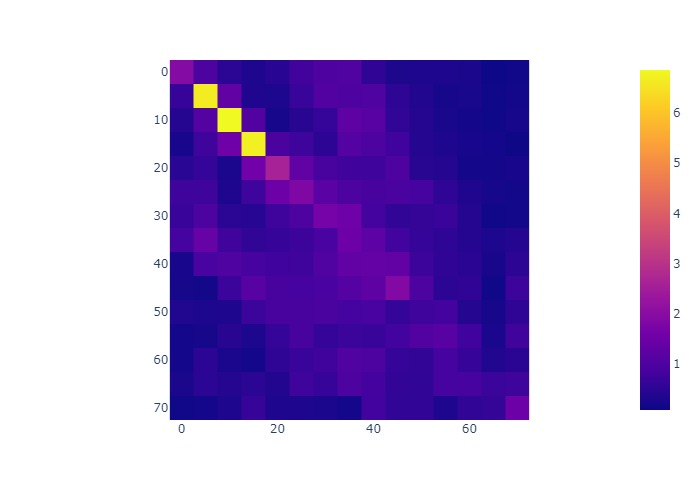
\includegraphics[width=350px]{raw_matrix.jpg}%
\caption{Raw matrices from Great Britain POLYMOD. Values are contacts per person per day.}%
\end{figure}

%
Matrices were adjusted to account for the differences in the age distribution of the Australian population distribution in 2022 compared to the population of Great Britain in 2008. The matrices were adjusted by taking the dot product of the unadjusted matrices and the diagonal matrix containing the vector of the ratios between the proportion of the British and Australian populations within each age bracket as its diagonal elements. %


\begin{figure}%
\centering%
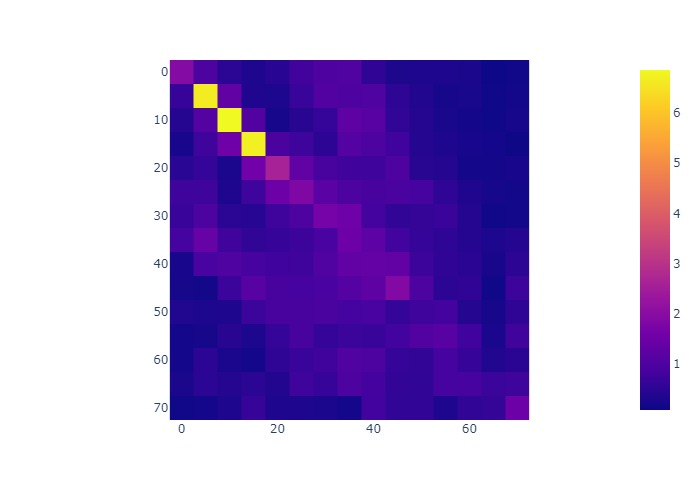
\includegraphics[width=350px]{adjusted_matrix.jpg}%
\caption{Matrices adjusted to Australian population. Values are contacts per person per day.}%
\end{figure}

%
We stratified all compartments of the base model into sequential age brackets in five year bands from age 0 to 4 through to age 65 to 69 with a final age band to represent those aged 70 and above. These age brackets were chosen to match those used by the POLYMOD survey. 

%
\section{Strain stratification}%
\label{sec:Strainstratification}%
We stratified the infectious compartment according to strain, including compartments to represent strains: BA.1 BA.2. This was implemented using summer's `StrainStratification' class. All of the starting infectious seed was assigned to the BA.1 category within the infectious category. %
The relative infectiousness of the BA.2 strain was adjusted relative to the starting strain (BA.1) as indicated in the parameters table. %
Each strain (including the starting wild{-}type) is seeded through a step function that allows the introduction of a constant rate of new infectious persons into the system over a fixed seeding duration. 

%
\section{Calibration}%
\label{sec:Calibration}%
Input parameters varied through calibration with uncertainty distribution parameters and support. \newline%
%
\begin{tabular}{p{2.7cm} p{2.7cm} p{2.7cm} p{2.7cm} }%
\hline%
\textbf{Name}&\textbf{Distribution}&\textbf{Distribution parameters}&\textbf{Support}\\%
\hline%
Rate of effective contacts&Uniform distribution&loc: 0.02 scale: 0.030000000000000002&0.02 to 0.05\\%
\hline%
Infectious period&Uniform distribution&loc: 4.0 scale: 4.0&4.0 to 8.0\\%
\hline%
\end{tabular}%
\linebreak%
\begin{tabular}{p{1.3cm} p{1.3cm} p{1.3cm} p{1.3cm} p{1.3cm} p{1.3cm} p{1.3cm} }%
\hline%
\textbf{Para{-}meter}&\textbf{Mean (SD)}&\textbf{3{-}97\% high{-}density interval}&\textbf{MCSE mean (SD)}&\textbf{ESS bulk}&\textbf{ESS tail}&\textbf{R\_hat}\\%
\hline%
Rate of effective contacts&0.021 (0.0)&0.021 to 0.021&0.0 (0.0)&1.0&1.0&nan\\%
\hline%
Infectious period&6.749 (0.105)&6.463 to 6.804&0.063 (0.051)&1.0&5.0&nan\\%
\hline%
\end{tabular}%
\linebreak%


\begin{figure}%
\centering%
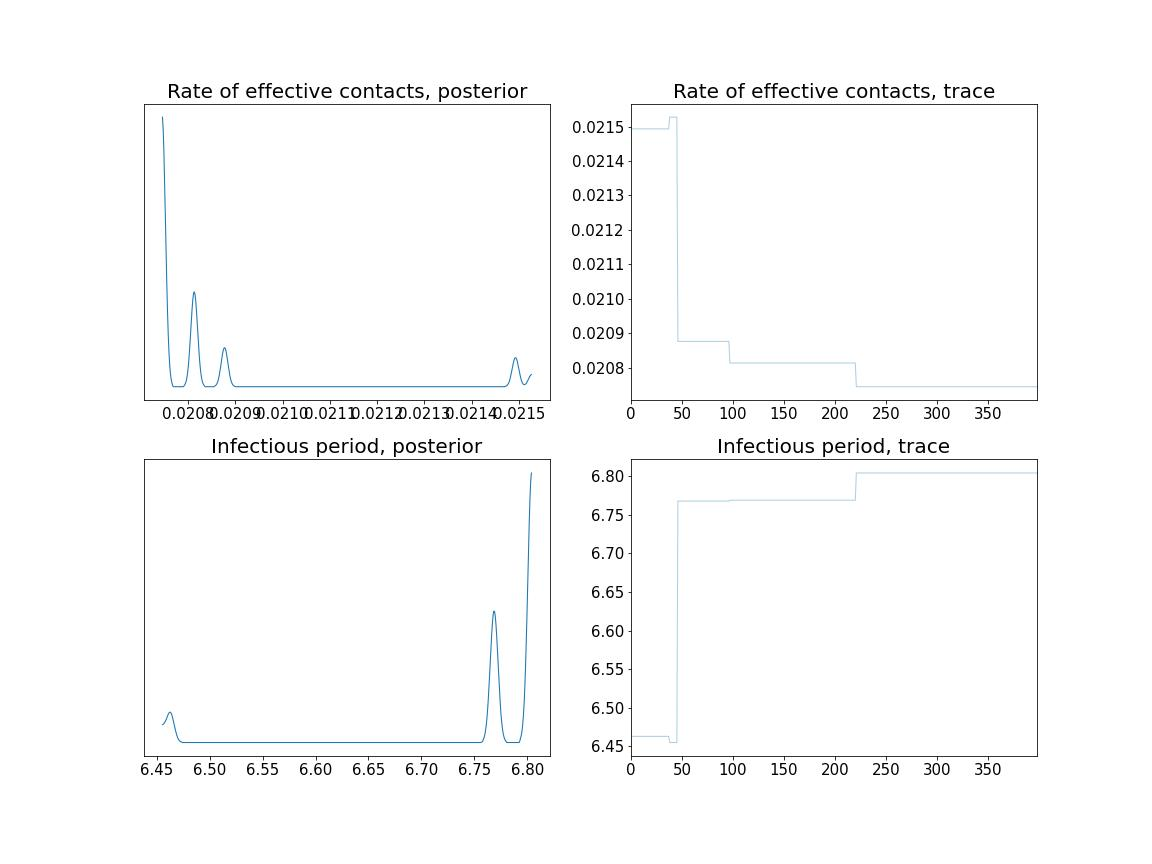
\includegraphics[width=350px]{progression.jpg}%
\caption{Parameter posteriors and progression.}%
\end{figure}

%
\begin{tabular}{p{2.7cm} p{2.7cm} p{5.8cm}}%
\hline%
\textbf{Name}&\textbf{Value}&\textbf{Evidence}\\%
\hline%
Rate of introduction of persons infected with each new variant&1.0 persons per day&Assumed\\%
\hline%
Relative infectiousness of BA.2 relative to BA.1&3.0 &Assumed\\%
\hline%
Time BA.2 infectious seed begins&750.0 &Assumed\\%
\hline%
Infectious period&Calibrated, see priors table&This quantity is difficult to estimate, given that identified cases are typically quarantined. Studies in settings of high case ascertainment and an effective public health response have suggested a duration of greater than 5.5 days \cite{bi2020}. PCR positivity, which may continue for up to two to three weeks from the point of symptom onset \cite{he2020} \cite{byrne2020} does not necessarily indicate infectiousness. The duration infectious for asymptomatic persons has also been estimated at 6.5 to 9.5 days \cite{byrne2020}.\\%
\hline%
Rate of effective contacts&Calibrated, see priors table&Calibrated within plausible range\\%
\hline%
Duration of introduction of persons infected with each new variant&1.0 days&Assumed\\%
\hline%
Case detection rate (proportion of infections captured through surveillance)&0.2 &Assumed\\%
\hline%
Time BA.1 infectious seed begins&600.0 &Assumed\\%
\hline%
\end{tabular}%
\linebreak

%
\section{Parameterisation}%
\label{sec:Parameterisation}%
Parameter interpretation, with value (for parameters not included in calibration algorithm) and summary of evidence. \newline%

%
\newpage%
\printbibliography%
\end{document}